\documentclass[t, notes, xcolor=table]{beamer}

\usepackage{wrapfig}
\usepackage{float}
% For tabs in verbatim
\usepackage{fancyvrb}

% Adjust position of the image
\usepackage[export]{adjustbox}

% set fonts
\usefonttheme{professionalfonts} % using non standard fonts for beamer
\usepackage{txfonts,mathptmx}

% set indend spacing for first and second level indentation
\setlength{\leftmargini}{0.5cm}
\setlength{\leftmarginii}{0.5cm}
\setlength{\leftmarginiii}{0.5cm}

% Set circles for bullets 
\setbeamertemplate{itemize items}[circle]

% colors
\usepackage{xcolor}

% multiple columns
\usepackage{multicol}

% todo lists
\usepackage{pifont}
\usepackage{amssymb}

% increase space between text and frame name
\addtobeamertemplate{frametitle}{}{\vspace{0.5em}}

%Information to be included in the title page:
\title{Coding RTL for Synthesis}
\author{Nikola Petrovic}
\institute{University of Belgrade, School of Electrical Engineering}
\date{2022}



\begin{document}

\frame{\titlepage}

%%%%%%%%%%%%%%%%%%%%%%%%%%%%%%%%%%%%%%%%%%%%%%%%%%%%%%%%%%%%
\begin{frame}
\frametitle{Module Objective}
In this module we will code design behaviour for logic synthesis.
\newline

\textbf{Topics:}
\begin{itemize}
\item Modeling combinational logic
\item Modeling sequential logic
\item Modeling latch logic
\item Modeling three-state logic
\item Using synthesis attributes
\end{itemize}
\end{frame}
\note{
\scriptsize{
Our objective is to code design behaviours for logic synthesis.
\newline

To do that, we need to know about:
\begin{itemize}
\item Modeling combinational logic
\item Modeling sequential logic
\item Modeling latch logic
\item Modeling three-state logic
\item Using synthesis attributes
\end{itemize}

}
}

%%%%%%%%%%%%%%%%%%%%%%%%%%%%%%%%%%%%%%%%%%%%%%%%%%%%%%%%%%%%
\begin{frame}
\frametitle{Modeling Combinational Logic}
Combinational Logic: Output is at all times a combinational function solely of the inputs.
\scriptsize{
\begin{multicols}{2}
\begin{itemize}
\item As a \textbf{net declaration} assignment
\item As a \textbf{continuous} assignment
\item As an \textbf{always} statement
\end{itemize}
\vfill
\columnbreak
\begin{figure}
    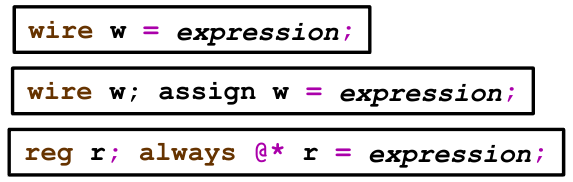
\includegraphics[width=0.45\textwidth]{img/13_seq_1.png}
\end{figure}
\end{multicols}
\begin{itemize}
\item The event list must not contain a posedge or negedge event.
\begin{itemize}
	\scriptsize{
	\item[$-$] Include all procedure inputs to avoid mismatch between pre-synthesis and post-synthesis designs.	
	}
\end{itemize}
\item Assignments must be blocking, they are sufficient and simulate more efficiently.
\end{itemize}
}
\begin{figure}
    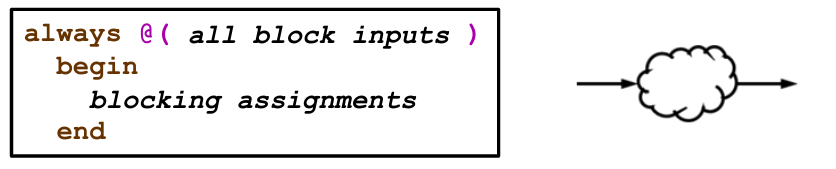
\includegraphics[width=0.75\textwidth]{img/13_seq_2.png}
\end{figure}
\end{frame}
\note{
\tiny{
We can model combinational logic with a net declaration assignment or a continuous assignment or an \textit{always} statements.
\newline

When using an \textit{always} statement, the single event list must not contain a \textit{posedge} or \textit{negedge} event. The event list does not otherwise affect the synthesis results, but to avoid incorrect RTL simulation results, we should include in the event list all inputs to the procedure. The easiest way to ensure this is to use the Verilog 2001 wild-card event control (@*).
\newline

We must not in an \textit{always} statement assign a variable using both a blocking and a non-blocking assignment The blocking assignment is sufficient for a description of combinational logic and simulates more efficiently than the non-blocking assignment.
\newline

\textbf{From IEEE Std. 1364.1-2002} \textit{Section 5.1}:

Combinational logic shall be modeled using a continuous assignment or a net declaration assignment or an
always statement.
\newline

When using an always statement, the event list shall not contain an edge event (posedge or negedge). The
event list does not affect the synthesized netlist. However, it may be necessary to include in the event list all
the variables read in the always statement to avoid mismatches between simulation and synthesized logic.
\newline

A variable assigned in an always statement shall not be assigned using both a blocking assignment (=) and a
nonblocking assignment (\textless=) in the same always statement.
\newline

The event list for a combinational logic model shall not contain the reserved words posedge or negedge. Not
all variables that appear in the right hand side of an assignment are required to appear in the event list. For
example, a variable does not have to appear in the event list of an always statement if it is assigned a value
with a blocking assignment before being used in subsequent expressions within the same always statement.
\newline

The event list may be the implicit event expression list (@(*), @*). 

}
}

%%%%%%%%%%%%%%%%%%%%%%%%%%%%%%%%%%%%%%%%%%%%%%%%%%%%%%%%%%%%
\begin{frame}
\frametitle{Incomplete Event List}
\scriptsize{
\begin{itemize}
\item For simulation, include in the event list all signals that are input to the logic.
\item The "*" wild-card sensitivity list automatically includes all input signals to the logic.
\end{itemize}
}
\begin{figure}
    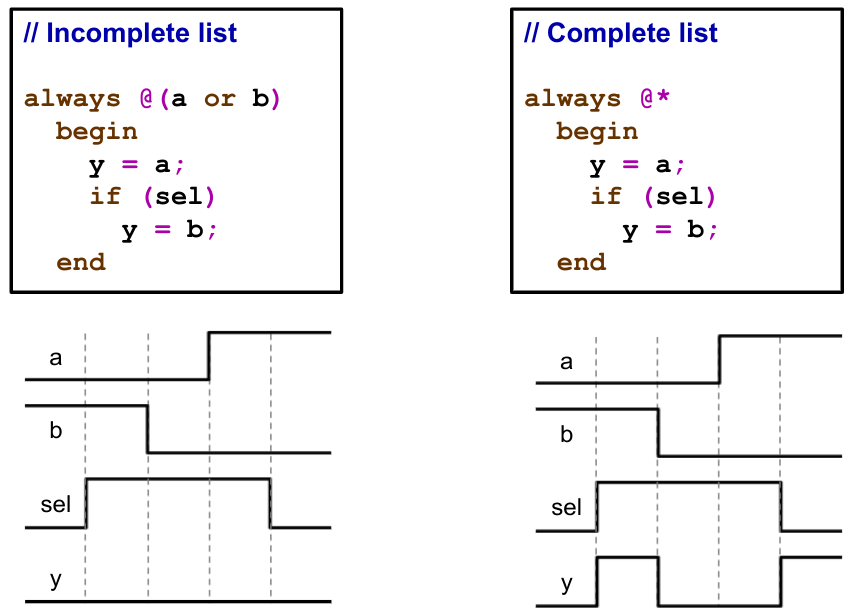
\includegraphics[width=0.65\textwidth]{img/13_event.png}
\end{figure}
\end{frame}
\note{
\scriptsize{
The event list does not affect the synthesis result, but to avoid incorrect RTL simulation results, we should include in the event list all inputs to the procedure. The easiest way to ensure this is to use the Verilog 2001 wildcard event control \textbf{(@*)}.
\newline

This example illustrates the affect of an incomplete sensitivity list.
\begin{itemize}
\item If the event list omits the \textit{sel} signal, the procedure executes upon transitions of only the \textit{a} and \textit{b} inputs - transitions of the \textit{sel} signal have no effect.
\item Debugging problems caused by an incomplete sensitivity list is difficult, so we might want to develop the habit of simply always using the wildcard event control for all combinational procedures.
\end{itemize}

\textbf{From IEEE Std. 1364.1-2002} \textit{Section 5.1}:

"The event list does not affect the synthesized netlist."

}
}

%%%%%%%%%%%%%%%%%%%%%%%%%%%%%%%%%%%%%%%%%%%%%%%%%%%%%%%%%%%%
\begin{frame}
\frametitle{Complete Event List}
\scriptsize{
\begin{multicols}{2}
The event list for a combinational procedure should contain all inputs to the logic.
\begin{figure}
    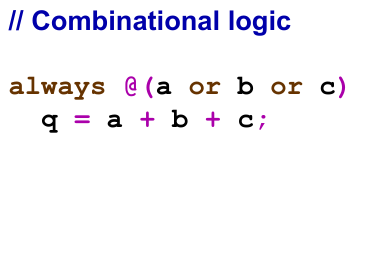
\includegraphics[width=0.35\textwidth,left]{img/13_complete_event_1.png}
\end{figure}
\vfill
\columnbreak
Do not include temporary variables in the sensitivity list.
\begin{figure}
    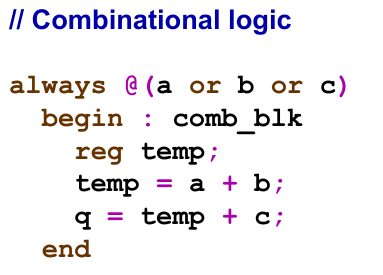
\includegraphics[width=0.35\textwidth,left]{img/13_complete_event_2.png}
\end{figure}
\end{multicols}
}
\end{frame}
\note{
\tiny{
The Verilog language let us place any signals in the sensitivity list and to freely mix blocking and non-blocking assignments anywhere in the procedure. A simulation tool simply executes the procedure as we wrote it, using simulation semantics.
\newline

However, to generate RTL simulation results consistent with those of the post-synthesis netlist, some guidelines exist:
\begin{itemize}
\item All edges of all signals input to combinational logic must be present in the sensitivity list. This is due to the rule that any changes on any input to the logic must have the opportunity to immediately affect the output. \textbf{Do not place temporary variables in the sensitivity list!} A temporary variable is one that the procedure writes only before it reads and that no other procedure uses. It is not an input to the logic.
\item Do not mix blocking and non-blocking assignments to the same variable. Even better, we should use only blocking assignments within procedures that represent purely combinational logic. This is a recommendation to obtain higher simulation performance, as non-blocking assignments are not necessary and simulate more slowly.
\end{itemize}
The synthesis tool requires code that unambiguously states our design intentions. Code meant for the synthesis tool may use only a subset of the Verilog constructs and coding styles.
\begin{itemize}
\item For synthesis, it is an absolute requirement that we don't mix blocking and non-blocking assignments to the same variable!
\item The synthesis standard states that the sensitivity list shall not affect the generation of combinational logic. That means that if the synthesis tool recognizes the block as combinational logic, it will proceed as if we had included all inputs to the logic in the sensitivity list. The synthesis tool may or may not warn us about missing inputs. The generated gates will simulate correctly, but very likely differently that the incorrect RTL simulation.
\end{itemize}

}
}

%%%%%%%%%%%%%%%%%%%%%%%%%%%%%%%%%%%%%%%%%%%%%%%%%%%%%%%%%%%%
\begin{frame}
\frametitle{Incomplete Assignments}
\textbf{Combinational Logic}
\footnotesize{
\begin{itemize}
\item Output is at all times a combinational function solely of the inputs.
\end{itemize}
}
\begin{figure}
    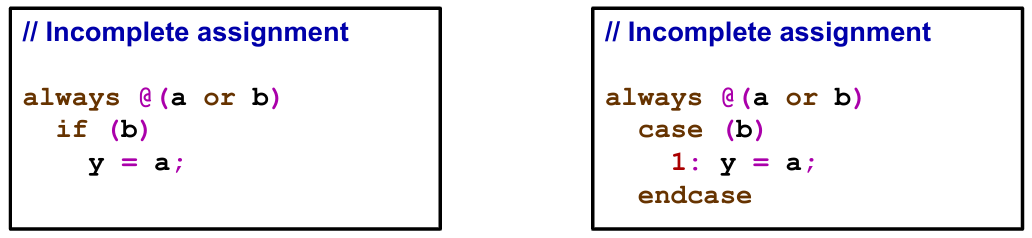
\includegraphics[width=0.95\textwidth]{img/13_incomplete_assign.png}
\end{figure}
\vfill

* What is the value of y when b is 0?
\end{frame}
\note{
\scriptsize{
If an execution path through a combinational procedure exists that does not update the value of some output, then the output variable must retain its previous state. The synthesis tool infers a latch to implement this behaviour. Latch inference is almost always non intended, and we can easily avoid it.
\newline

This example fails to update the \textit{y} output variable when the input \textit{b} is not 1.
\newline

How would you modify this code to ensure inference of purely combinational logic?

}
}

%%%%%%%%%%%%%%%%%%%%%%%%%%%%%%%%%%%%%%%%%%%%%%%%%%%%%%%%%%%%
\begin{frame}
\frametitle{Complete Assignment}
Avoiding latch inference is easy!
\footnotesize{
\begin{itemize}
\item Provide outputs with a value for every combination of inputs.
\item This is most easily done with default assignments.
\end{itemize}
}
\begin{figure}
    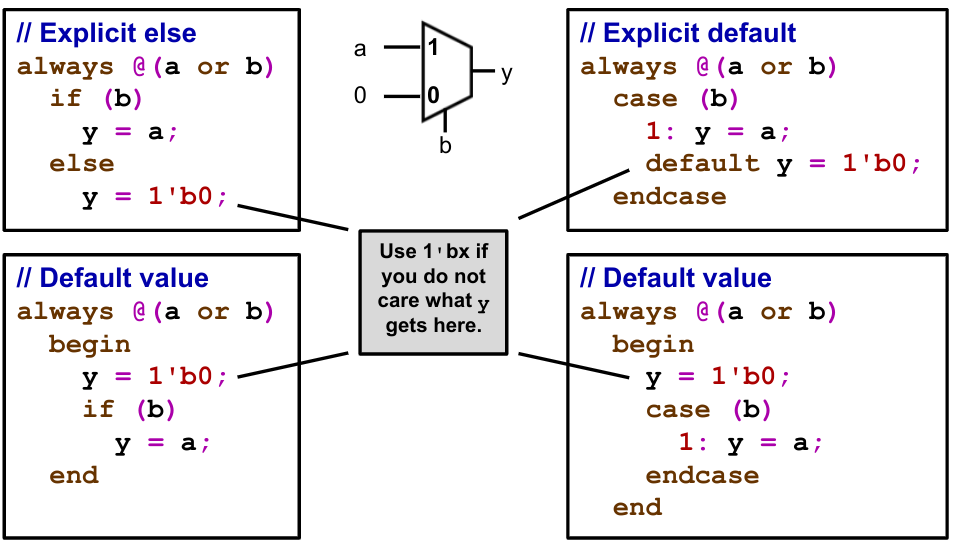
\includegraphics[width=0.75\textwidth]{img/13_complete_assign.png}
\end{figure}
\end{frame}
\note{
\scriptsize{
Here are two methods we can use to prevent latch inference:
\begin{itemize}
\item We can for an \textit{if} statement use an explicit \textit{else} clause and for a \textit{case} statement an explicit default match item.
\item we can provide default values for all procedure outputs at the start of the procedure.
\end{itemize}
Which is the best technique in a real design?
\newline

If we have a procedure with a complex set of conditional assignments, we can easily miss an assignment for one or more of these branches. Making default assignments at the start of the procedure ensures that all procedure outputs have an assignment.
\newline

\textbf{From IEEE Std. 1364.1-2002} \textit{Section 5.5} Support for values x and z:

The value \textbf{x} may be used as a primary on the RHS of an assignment to indicate a don't care value for synthesis.

}
}

%%%%%%%%%%%%%%%%%%%%%%%%%%%%%%%%%%%%%%%%%%%%%%%%%%%%%%%%%%%%
\begin{frame}
\frametitle{Continuous Assignments}
Continuous assignments drive values onto nets.
\newline

Continuous assignments always represent combinational logic.
\begin{itemize}
\item Impossible to not assign a value for some input combination.
\item Output is always a combinational function of current inputs.
\end{itemize}
\vspace{10pt}
\begin{figure}
    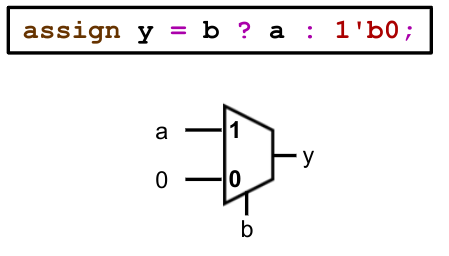
\includegraphics[width=0.45\textwidth]{img/13_cont_assign.png}
\end{figure}
\end{frame}
\note{
\scriptsize{
Continuous assignments and net declaration assignments drive values onto nets. These assignments always represent combinational logic, as it is syntactically impossible to not assign a value for some input combination, thus the output is always a combinational function of the current inputs.

}
}

%%%%%%%%%%%%%%%%%%%%%%%%%%%%%%%%%%%%%%%%%%%%%%%%%%%%%%%%%%%%
\begin{frame}
\frametitle{Modeling Combinational Logic Summary}
\footnotesize{
Summary of the steps to procedurally describe purely combinational logic:
\begin{itemize}
\item Start the procedure with the \textbf{always} construct.
\item Immediately follow the always construct with an event control.
\begin{itemize}
	\scriptsize{
	\item[$-$] Place all possible input events in the event expression.	
	}
\end{itemize}
\item Group multiple following statements with \textbf{begin...end} block.
\item Provide default assignments to prevent latch inference.
\item Avoid combinational feedback loops.
\item Assign a variable in only one procedure.
\end{itemize}
}
\end{frame}
\note{
\scriptsize{
Here is a summary of the steps to procedurally describe purely combinational logic:
\begin{itemize}
\item Start the procedure with the \textbf{always} construct.
\item Immediately follow the always construct with an event control. Place all possible input events in the event expression.	
\item Group multiple following statements with \textbf{begin...end} block. We can omit the \textbf{begin...end} keywords if we have only a single statement.
\item make blocking assignments. We can equally validly make non-blocking assignments, but they simulate less efficiently and provide no additional benefit. In any case, do NOT mix blocking and non-blocking assignments to the same variable and do NOT make assignments to a variable from multiple procedures.
\item Provide default assignments to prevent latch inference.
\item Avoid combinational feedback loops.
\end{itemize}
Remember that:
\begin{itemize}
\item Continuous assignments always synthesize to combinational logic.
\item Functions almost always synthesize to combinational logic.
\end{itemize}
}
}

%%%%%%%%%%%%%%%%%%%%%%%%%%%%%%%%%%%%%%%%%%%%%%%%%%%%%%%%%%%%
\begin{frame}
\frametitle{Modeling Sequential Logic}
\textbf{Sequential Logic}
\newline

\footnotesize{
\begin{itemize}
\item Outputs are sampled in registers on a clock edge, thus storage is required.
\item As an always statement:
\begin{itemize}
	\footnotesize{
	\item The event list must contain only posedge and negedge events.
	\item Model set/reset behaviours in an if statement early branches and normal behaviour in the later branches.
	\item Make non-blocking assignments to storage variables.	
	}
\end{itemize}
\end{itemize}
}
\vspace{20pt}
\begin{figure}
    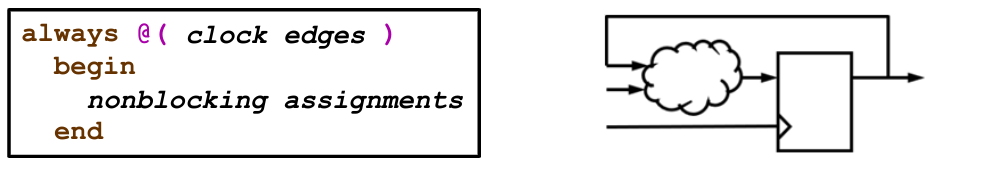
\includegraphics[width=0.75\textwidth]{img/13_seq_logic.png}
\end{figure}

\end{frame}
\note{
\scriptsize{
We model sequential logic using an \textit{always} statement that has one or more \textit{posedge} or \textit{negedge} events in exactly one event list. Exactly one of those events represents the active clock edge that stores the value. Any additional \textit{posedge} or \textit{negedge} events represent asynchronous set and reset behaviours. The event list must NOT contain level-sensitive events.
\newline

We model the asynchronous set and reset behaviours by using an \textit{if} statement in the \textit{if} statement, we model the asynchronous behaviours in one or more conditional branches. The unconditional last \textit{else} branch models the normal sequential behaviour.
\newline

To avoid simulation clock/data races, we should make only non-blocking assignments to variables that represent storage. We make blocking assignments to temporary variables. Temporary variables are those written and then read in the same procedure and nowhere else.

}
}

%%%%%%%%%%%%%%%%%%%%%%%%%%%%%%%%%%%%%%%%%%%%%%%%%%%%%%%%%%%%
\begin{frame}
\frametitle{Normal Behaviour}
\scriptsize{
\begin{multicols}{2}
The event list for a sequential procedure must contain only single edges of clock signals.
\begin{itemize}
\item All events must be posedge or negedge qualified.
\end{itemize}
The synthesis tool infers registers:
\begin{itemize}
\item For non-temporary variables assigned in sequential procedures:
\begin{itemize}
	\scriptsize{
	\item[$-$] Assigned with non-blocking statements	
	}
\end{itemize}
\end{itemize}
\vfill
\columnbreak
\begin{figure}
    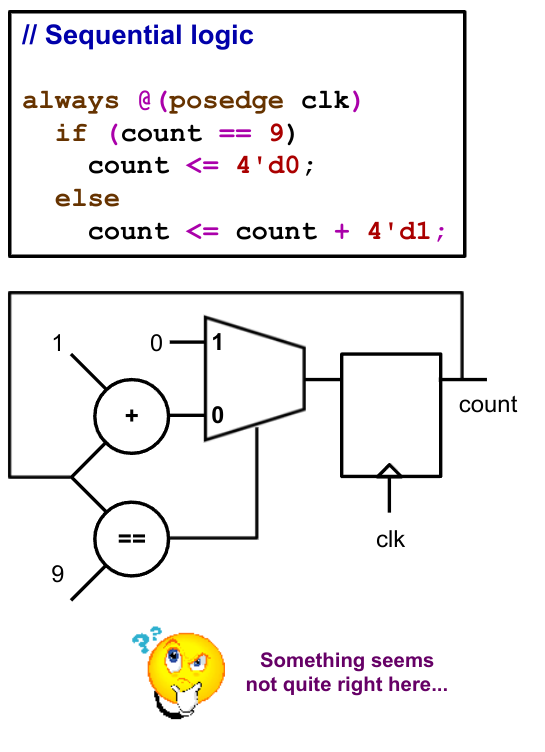
\includegraphics[width=0.45\textwidth]{img/13_seq_normal.png}
\end{figure}
\end{multicols}
}
\end{frame}
\note{
\scriptsize{
Synthesis tools recognize sequential procedures by looking for a particular code template - in this case, a procedure with an event list containing only edge-qualified signals. Although some synthesis tools may support other coding styles for sequential procedures, our adherence to this standard produces code that we can port between all synthesis tools compliant with the standard.
\newline

This example has only the positive edge of the clock in its event list. All storage inferred for non-temporary variables that this procedure writes will have a rising active clock edge. The \textit{if} statement describes the combinational logic calculating the new "count" value that is stored on the nest rising clock edge.
\newline

\textbf{Note that this example lacks a reset to initialize the count value!}

}
}

%%%%%%%%%%%%%%%%%%%%%%%%%%%%%%%%%%%%%%%%%%%%%%%%%%%%%%%%%%%%
\begin{frame}
\frametitle{Reset Behaviour}
Use an \textbf{if...else} statement to add set/reset to a procedure.
\footnotesize{
\begin{itemize}
\item Put the set/reset behaviour in the first branch.
\item Put the normal sequential behaviour in the last branch.
\item For asynchronous resets, add active set/reset edges to event list.
\end{itemize}
}
\vfill
\begin{figure}
    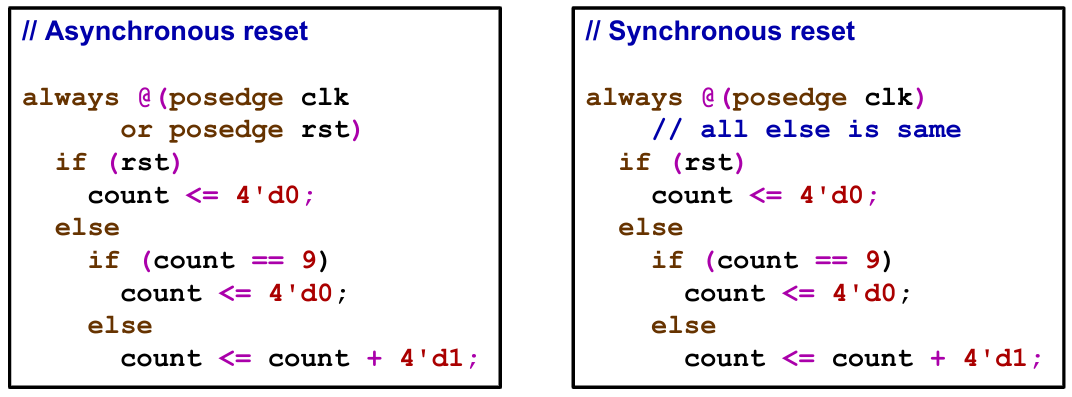
\includegraphics[width=0.95\textwidth]{img/13_seq_reset.png}
\end{figure}
\end{frame}
\note{
\scriptsize{
We can most easily provide set and reset behaviours by using an \textit{if} statement. This is a requirement for asynchronous set and reset behaviours and strongly recommended for synchronous set and reset behaviours. The synthesis tool will tread synchronous set and reset behaviours we model outside an \textit{if} statement as just that much more combinational logic.
\newline

If the \textit{if} statement, place the set and reset behaviours in their order of priority in the first conditional branches, and place the normal synchronous behaviour in the unconditional last \textit{else} branch. Do NOT make assignments to the storage variable outside of the \textit{if} statement.
\newline
For synchronous set and reset, trigger the procedure on only the clock edge/
\newline

For asynchronous set and reset, trigger the procedure also on the active set and reset edge(s).
\newline
Code synchronously reset, asynchronously reset and non reset registers in separate procedures.

}
}

%%%%%%%%%%%%%%%%%%%%%%%%%%%%%%%%%%%%%%%%%%%%%%%%%%%%%%%%%%%%
\begin{frame}
\frametitle{Sequential Procedure Templates}
Code must follow these templates:
\footnotesize{
\begin{itemize}
\item Procedure starts with an always construct.
\item Followed by one event control containing only edge-qualified signals.
\begin{itemize}
\footnotesize{
	\item[$-$] Clock
	\item[$-$] Asynchronous set or reset
	}
\end{itemize}
\end{itemize}
}
\vfill
\begin{figure}
    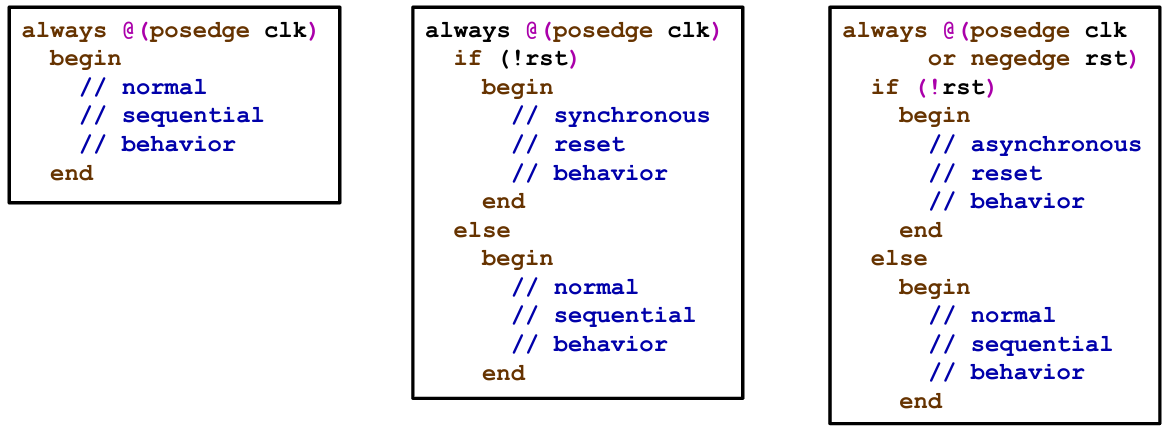
\includegraphics[width=0.95\textwidth]{img/13_seq_template.png}
\end{figure}
\end{frame}
\note{
\scriptsize{
Sequential procedures have the clock edge in the event list, and also the set and reset edge(s) if there is asynchronous set or reset.
\newline

Separately code your non reset, synchronous reset and asynchronous reset procedures.

}
}

%%%%%%%%%%%%%%%%%%%%%%%%%%%%%%%%%%%%%%%%%%%%%%%%%%%%%%%%%%%%
\begin{frame}
\frametitle{Incomplete Assignments}
\footnotesize{

\textbf{Sequential Logic}
\begin{itemize}
\item Output is not at all times a combinational function solely of the inputs.
\begin{itemize}
	\scriptsize{
	\item[$-$] Implies some kind of storage
	}
\end{itemize}
\item Incomplete assignment in a sequential procedure does not infer a latch.
\begin{itemize}
	\scriptsize{
	\item[$-$] Storage is already there!
	}
\end{itemize}
\end{itemize}

\begin{figure}
    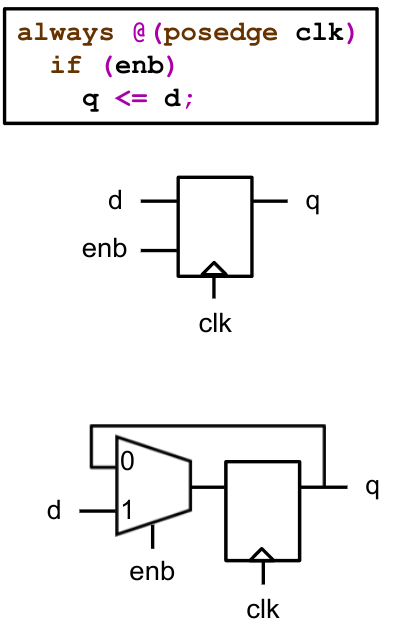
\includegraphics[width=0.3\textwidth]{img/13_seq_incomplete.png}
\end{figure}

}
\end{frame}
\note{
\scriptsize{
If procedure execution does not update a variable, then the variable value is not changed. In procedures representing combinational logic, this infers a latch to store a previous variable value. For procedures representing synchronous logic, the variable value is stored in the inferred register. For these procedures we do not use default assignment or \textit{else} clauses to prevent latch inference.

}
}

%%%%%%%%%%%%%%%%%%%%%%%%%%%%%%%%%%%%%%%%%%%%%%%%%%%%%%%%%%%%
\begin{frame}
\frametitle{Blocking vs. Non-blocking Assignment}
Write a Verilog sequential procedure to codify this behaviour.
\begin{figure}
    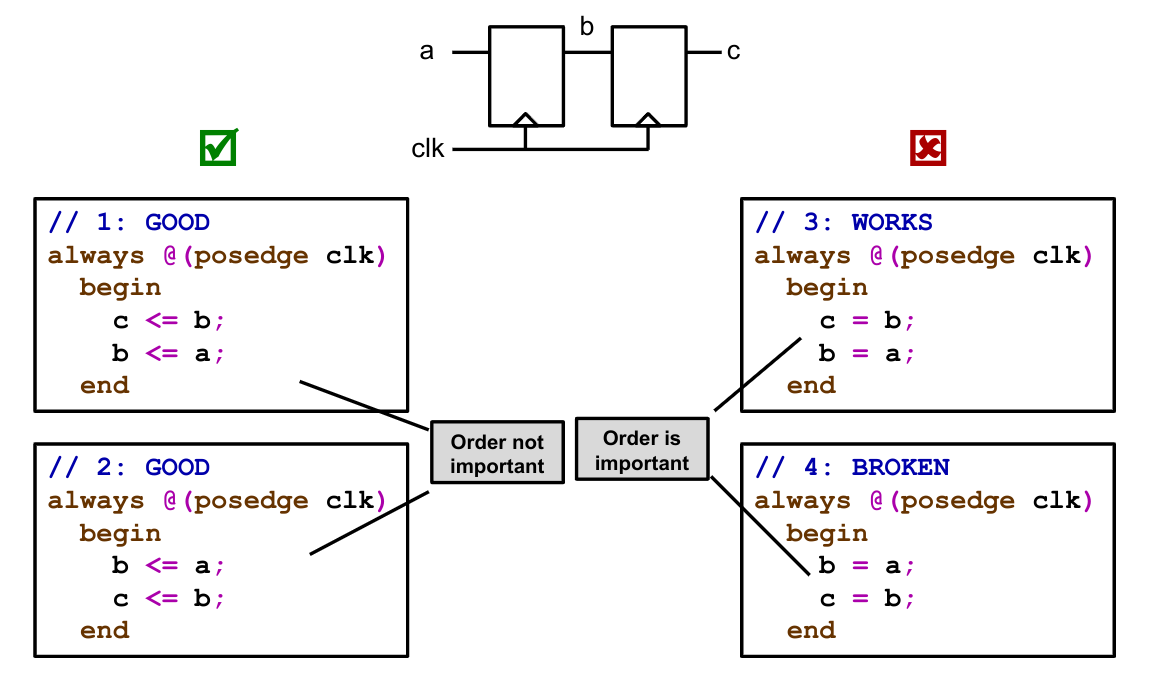
\includegraphics[width=0.95\textwidth]{img/13_block_vs_nonblock.png}
\end{figure}
\end{frame}
\note{
\scriptsize{
Good coding practice demands that we make only non-blocking assignments to variables that represent storage elements. This is to avoid clock/data races in simulation and to avoid unintended logic inference in synthesis. The synthesis standard requires only that we do not mix the two types of assignments to the same variable.
\newline

For examples 1 and 2, we can see that with non-blocking assignments the order of assignments is \textbf{not} important, as simulation schedules the actual assignments for the NBA region of the stratified event queue.
\newline

For examples 3 and 4, we can see that with blocking assignments the order of assignments \textbf{is} important, as the simulation completes the assignments as it executes the statements. Different order generates different simulation results and different synthesis results.
\begin{itemize}
\item Example 3 reads variable \textit{b} before writing it, so synthesis infers two registers.
\item Example 4 reads variable \textit{b} after writing it. Variable \textit{b} is temporary variable. Synthesis infers on register.
\end{itemize}

\textbf{From IEEE Std. 1364.1-2002} \textit{Section 5.2.2} Modeling edge-sensitive storage devices:

Non-blocking procedural assignments should be used for variables that model edge-sensitive storage devices.

}
}


%%%%%%%%%%%%%%%%%%%%%%%%%%%%%%%%%%%%%%%%%%%%%%%%%%%%%%%%%%%%
\begin{frame}
\frametitle{Temporary Variables in Sequential Procedures}

\scriptsize{
\begin{multicols}{2}
\textbf{Persistent Variable}
\begin{itemize}
\item Read first and then written (in the same procedure)
\item Synthesis must infer a register to hold a value to the next read.
\end{itemize}

\vfill
\columnbreak

\textbf{Temporary Variable}
\begin{itemize}
\item Written first and then read (in the same procedure)
\item Variable is alias for expression so no register is inferred
\end{itemize}

\end{multicols}
}
\begin{figure}
    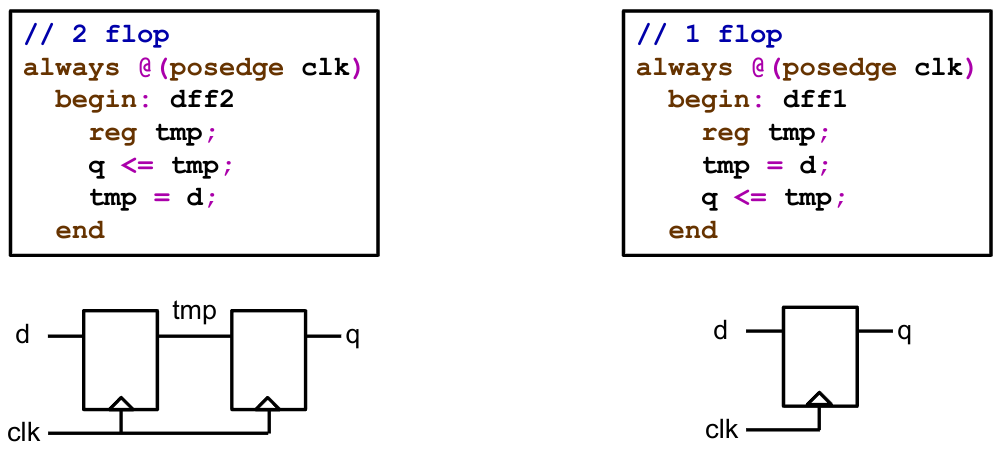
\includegraphics[width=0.95\textwidth]{img/13_temp_var.png}
\end{figure}
\end{frame}
\note{
\scriptsize{
We can use a temporary variable to hold intermediate result of a calculation before we use the result later in the procedure. We use temporary variables to break complex expressions and combinational logic into a series of smaller steps - making complex logic easier to describe, understand and maintain.
\newline

A temporary variable is one that a procedure writes with a blocking assignment only before the procedure reads it, and no other procedure uses it. We can declare temporary variables locally to ensure that no other procedure uses it.
\newline

A typical use model would be to make blocking assignments to temporary variables and the make non-blocking assignment of the temporary variable values to other variables.
\newline

\textbf{From IEEE Std. 1364.1-2002} \textit{Section 5.2.2} Modeling edge-sensitive storage devices:

Blocking procedural assignments may be used for variables that are temporary assigned and used within an always statement.

}
}

%%%%%%%%%%%%%%%%%%%%%%%%%%%%%%%%%%%%%%%%%%%%%%%%%%%%%%%%%%%%
\begin{frame}
\frametitle{Modeling Sequential Logic Summary}
\footnotesize{
Summary of the steps to procedurally describe sequential logic:
\begin{itemize}
\item Start the procedure with the \textit{always} construct.
\item Immediately follow the always construct with an event control.
\begin{itemize}
	\scriptsize{
	\item[$-$] Use only posedge or negedge events in the event expression.
	\item[$-$] Include only clock and asynchronous set/reset events.	
	}
\end{itemize}
\item Group multiple following statements within a \textit{begin...end} block.
\item Place the asynchronous set/reset behaviours firs (in their order of priority) in the \textit{if} statement.
Place the normal sequential behaviour in the last \textit{else} branch.
\begin{itemize}
	\scriptsize{
	\item[$-$] Make blocking assignments only to the temporary variables.
	\item[$-$] Make non-blocking assignments to the register variables.	
	}
\end{itemize}
\item Do not make assignments to a variable from multiple procedures.
\end{itemize}
}
\end{frame}
\note{
\scriptsize{
Here is a summary of the steps to procedurally describe sequential logic:
\begin{itemize}
\item Start the procedure with the \textit{always} construct. Immediately follow the always construct with an event control, placing only edge-qualified events in the event expression.
\item Group multiple following statements within a \textit{begin...end} block. We can omit the \textit{begin...end} keywords if we have only a single statement.
\item Make blocking assignments only to the temporary variables and make only non-blocking assignments to variables representing storage. Write the temporary variables only before you read them in the same procedure. Do not make assignments to a variable from multiple procedures.
\end{itemize}

}
}

%%%%%%%%%%%%%%%%%%%%%%%%%%%%%%%%%%%%%%%%%%%%%%%%%%%%%%%%%%%%
\begin{frame}
\frametitle{Modeling Latch Logic}
But what if we want to infer a latch?
\footnotesize{
\begin{itemize}
\item A combinational block that for some combination of inputs does not provide output value infers storage i.e., a latch.
\item Make assignments for latch logic as we do for sequential logic.
\begin{itemize}
	\scriptsize{
	\item[$-$] Make blocking assignments to only the temporary variables
	\item[$-$] Write temporary variables only before they are read
	\item[$-$] Make non-blocking assignments to the latch variable
	}
\end{itemize}
\end{itemize}
}
\begin{figure}
    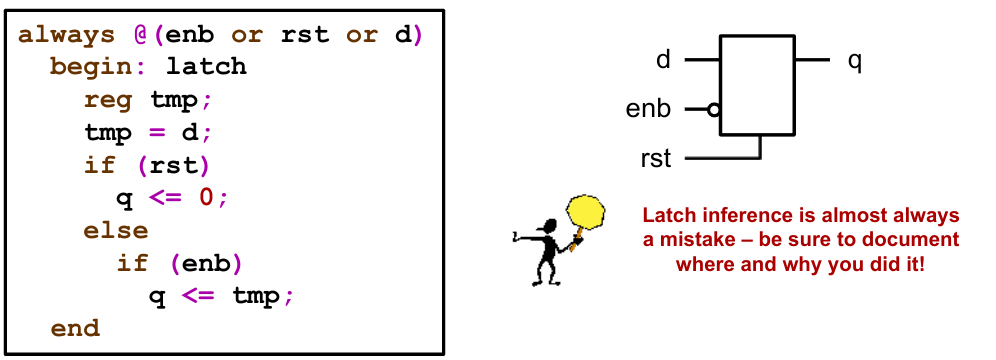
\includegraphics[width=0.75\textwidth]{img/13_latch.png}
\end{figure}
\end{frame}
\note{
\scriptsize{
We deliberately infer a latch, if we truly want to, the same way we inadvertently infer a latch, with the exception that we need to remember to make a non-blocking assignment to the variable that represents the latch.
\newline

A latch-based design can have higher performance than a register-based design, but can also be more difficult to correctly design and debug. Use of latches is typically infrequent and reserved for extenuating circumstances.

}
}

%%%%%%%%%%%%%%%%%%%%%%%%%%%%%%%%%%%%%%%%%%%%%%%%%%%%%%%%%%%%
\begin{frame}
\frametitle{Modeling Three-State Logic}
\begin{figure}
    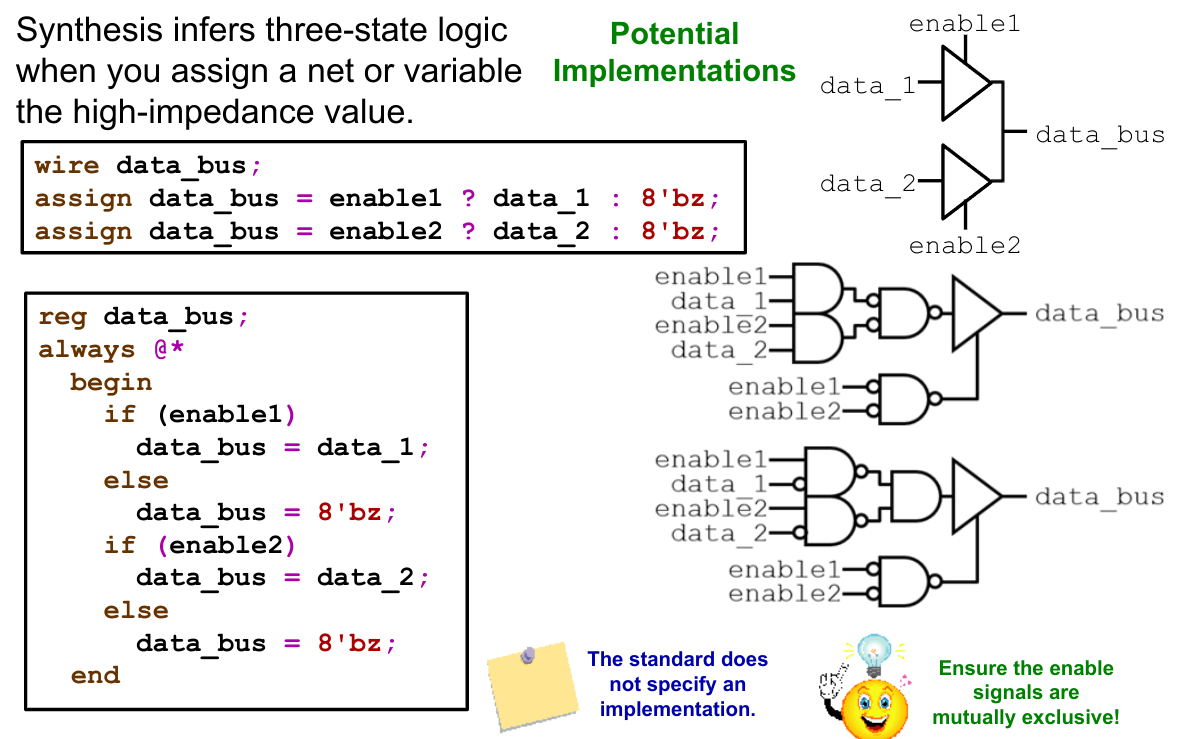
\includegraphics[width=0.95\textwidth]{img/13_three_state.png}
\end{figure}
\end{frame}
\note{
\scriptsize{
We model three-state logic by assigning the high-impedance value to a net or variable. Any other assignments to that net or variable must also assign the high-impedance value. Further propagating the high-impedance value by use of net or variable assignments does not also make that downstream logic into three-state logic.
\newline

This example codes behaviour representing three-state drivers in a form that synthesis can recognize. For this example:
\begin{itemize}
\item The "enable1" signal when high drives "data\_1" onto the data bus
\item The "enable2" signal when high drives "data\_2" onto the data bus.
\end{itemize}
The synthesis standard does not address what the result should be if multiple enables are simultaneously true.

}
}

%%%%%%%%%%%%%%%%%%%%%%%%%%%%%%%%%%%%%%%%%%%%%%%%%%%%%%%%%%%%
\begin{frame}[fragile]
\frametitle{Using Synthesis Attributes}
\footnotesize{
Verilog attributes provide supporting information about HDL items.

Verilog defines only the attribute syntax and where they may appear.

\begin{Verbatim}[commandchars=\\\{\}, tabsize=2]
\textcolor{purple}{	(* name [= const_expr] \{, name [= const_expr] \} *)}
\end{Verbatim}
\begin{itemize}
\item Does not define any attribute names or values
\end{itemize}

The synthesis standard defines some attributes and their purpose.
\begin{itemize}
\item For some the standard does not define what values to accept
\end{itemize}

Synthesis vendors add their own attributes.
\begin{itemize}
\item Also other pragmas in the form of metacomments
\end{itemize}
}
\begin{figure}
    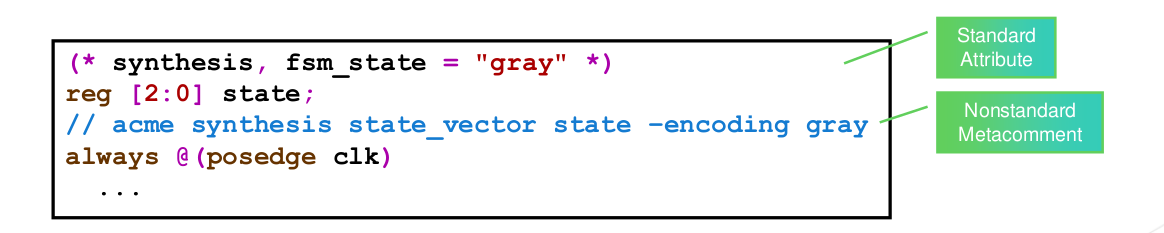
\includegraphics[width=0.95\textwidth]{img/13_attributes.png}
\end{figure}
\end{frame}
\note{
\tiny{
The IEEE Std. 1364-2001 Verilog HDL defines an attribute construct as a means to provide supporting
information about an HDL construct to the various tools reading the HDL. The Verilog standard defines only the
attribute syntax and where they may appear, and does not define any particular attributes.
\newline

The IEEE Std. 1364.1-2002 for Verilog RTL synthesis defines some synthesis attributes and requires that if a
compliant tool supports any means to provide this information then it must support provision my means of the
attributes.
\newline

As synthesis existed for many years prior to the Verilog RTL synthesis standard, synthesis vendors typically do
still offer their own means to provide this information as metacomments. The industry collectively refers to these
attributes and metacomments as “pragmas”.
\newline

This section will describe only a few of the standard synthesis attributes.
\newline

Attributes: “...properties about objects, statements and groups of statements in the HDL source...” – IEEE Std.
1364-2001 Section 2.8 Attributes
\newline

“An attribute instance can appear in the Verilog description as a prefix attached to a declaration, a module item, a
statement, or a port connection. It can appear as a suffix to an operator or a Verilog function name in an
expression.” – IEEE Std. 1364-2001 Section 2.8 Attributes
\newline

“A pragma is a generic term used to define a construct with no predefined language semantics that influences how
a synthesis tool should synthesize Verilog HDL code into a circuit.” – IEEE Std. 1364.1-2002 Section 6 Pragmas
\newline

“If a synthesis tool supports pragmas to control the structure of the synthesized netlist or to give direction to the
synthesis tool, attributes shall be used to convey the required information.” – IEEE Std. 1364.1-2002 Section 6.1
Synthesis attributes.

}
}

%%%%%%%%%%%%%%%%%%%%%%%%%%%%%%%%%%%%%%%%%%%%%%%%%%%%%%%%%%%%
\begin{frame}
\frametitle{Pragma “full\_case”}
\footnotesize{
\begin{itemize}
\item Synthesis tools accept a pragma to complete a \textbf{case} statement.
\item The directive applies to the case item expressions, not their statements!
\end{itemize}
}
\begin{figure}
    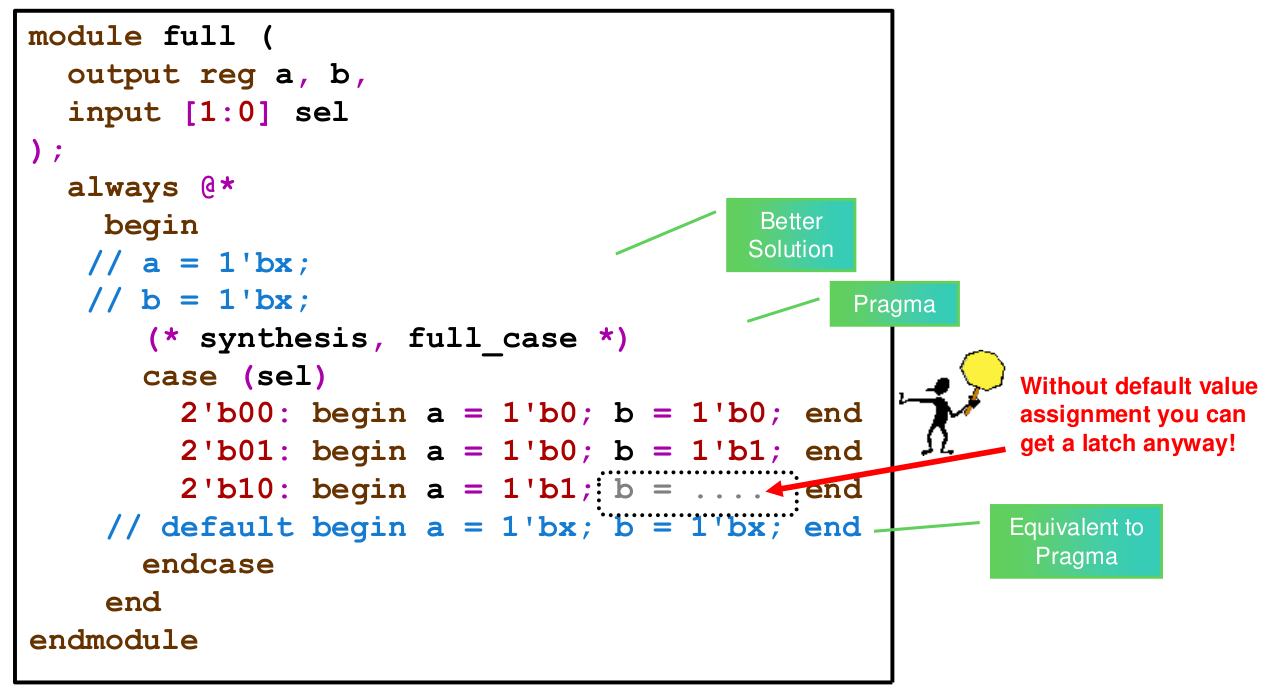
\includegraphics[width=0.95\textwidth]{img/13_pragma_full.png}
\end{figure}
\end{frame}
\note{
\scriptsize{
The full\_case attribute directs the synthesis tool to assign don't-care values to case statement outputs for
all unspecified case choices. Synthesis can still infer a latch for outputs not assigned by all specified
case items. Your use of the full\_case attribute thus promotes inadvertent errors. A better solution is to
explicitly provide default values for all procedure outputs.

}
}

%%%%%%%%%%%%%%%%%%%%%%%%%%%%%%%%%%%%%%%%%%%%%%%%%%%%%%%%%%%%
\begin{frame}
\frametitle{Pragma “parallel\_case”}
Synthesis tools accept a pragma to suppress the priority structure.
\vfill
\begin{figure}
    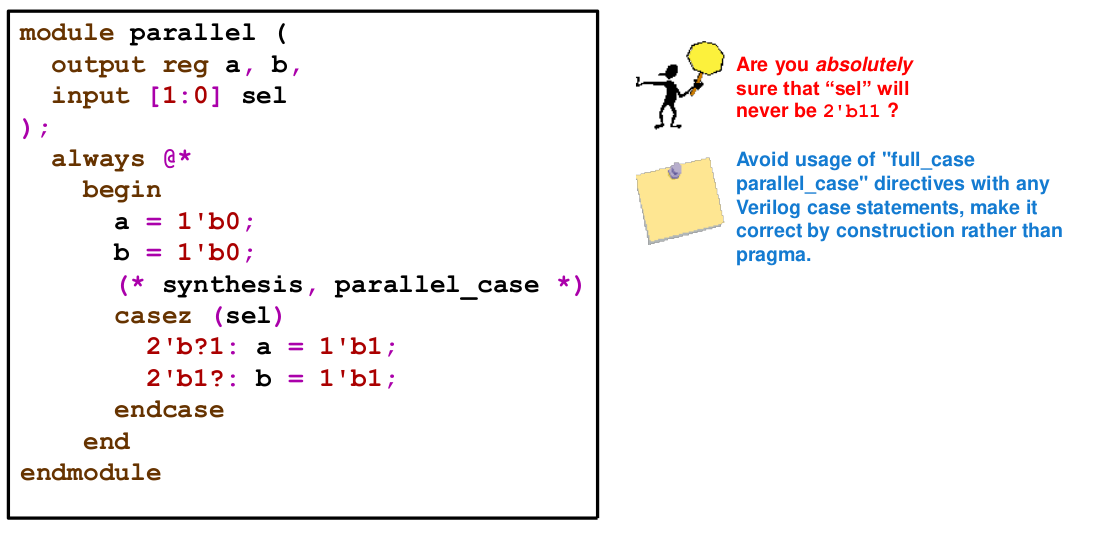
\includegraphics[width=0.95\textwidth]{img/13_pragma_parallel.png}
\end{figure}
\end{frame}
\note{
\scriptsize{
The parallel\_case attribute directs the synthesis tool to disregard the implied priority of the case items
and test all case items in parallel. This is in effect a declaration that the case items are mutually
exclusive in normal operation, and can produce a more optimal post-synthesis netlist. You must be very
careful to not declare case items to be mutually exclusive if they are not.

}
}

%%%%%%%%%%%%%%%%%%%%%%%%%%%%%%%%%%%%%%%%%%%%%%%%%%%%%%%%%%%%
\begin{frame}
\frametitle{Pragma “implementation”}
\scriptsize{
\begin{itemize}
\item Synthesis tools accept a pragma to recommend an operator architecture. The synthesis vendor defines the legitimate attribute values.
\end{itemize}
\begin{figure}
    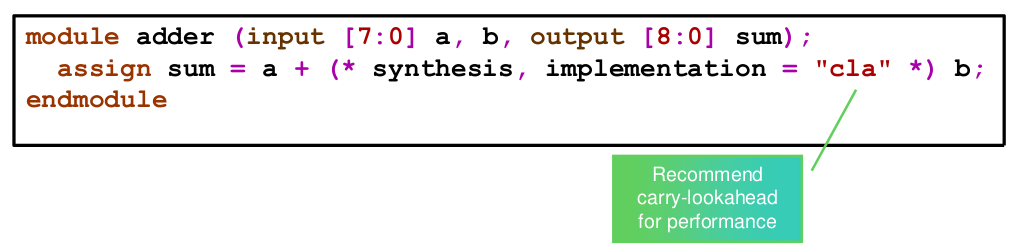
\includegraphics[width=0.95\textwidth]{img/13_pragma_implementation.png}
\end{figure}
\begin{itemize}
\item It is generally a good coding style to give the synthesis tool and simulator same information about the functionality of a design.
\end{itemize}
}
\end{frame}
\note{
\scriptsize{
\textbf{Make the code correct by construction rather than using pragma. (Pragmas can be found majorly in some legacy code.)}
\newline

The implementation attribute recommends an architecture for operator implementation. The synthesis vendor defines the legitimate values. The synthesis tool can legally ignore the recommendation.

}
}

%%%%%%%%%%%%%%%%%%%%%%%%%%%%%%%%%%%%%%%%%%%%%%%%%%%%%%%%%%%%
\begin{frame}
\frametitle{Pragma [a]sync\_set\_reset}
Synthesis tools accept a pragma to cause direct connection of set / reset signals to set / reset terminals and optionally designate set / reset signals.
\begin{figure}
    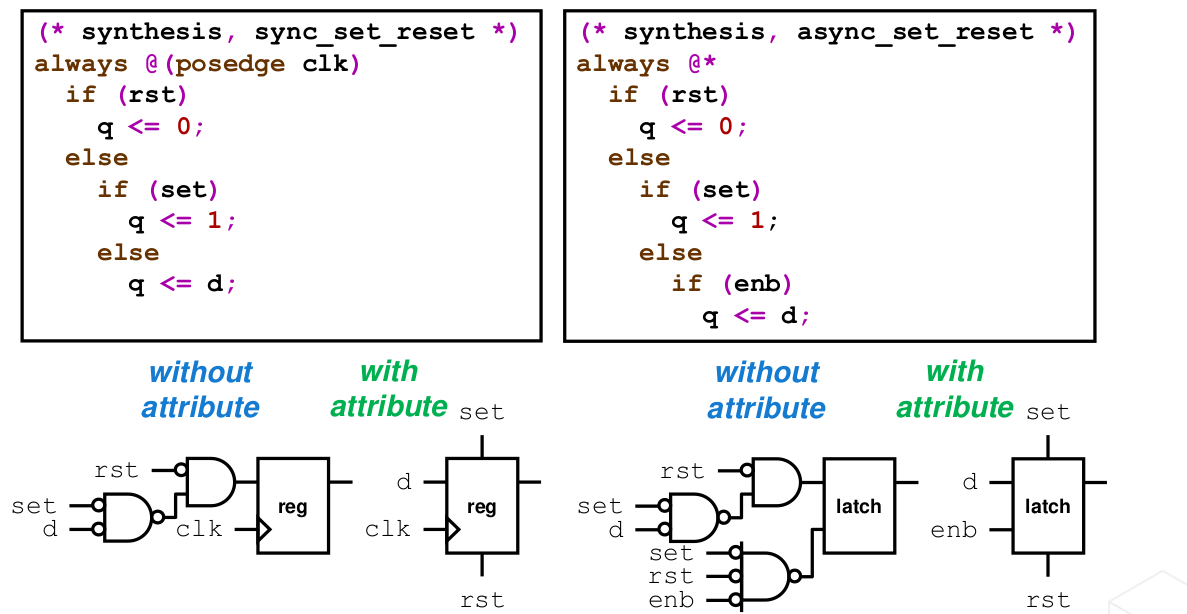
\includegraphics[width=0.95\textwidth]{img/13_pragma_async_reset.png}
\end{figure}
\end{frame}
\note{
\scriptsize{
The sync\_set\_reset attribute causes synthesis to directly connect synchronous set and reset signals to the
device set and reset terminals, if a device with such terminals exists in the library. You can apply this
attribute to a module or to a procedure. If you also designate the set or reset signals, then synthesis will
not directly connect any other set or reset signals to the device set and reset terminals, but will instead
route them into the data logic.
\newline

The async\_set\_reset attribute has exactly the same effect upon latch logic.

}
}

%%%%%%%%%%%%%%%%%%%%%%%%%%%%%%%%%%%%%%%%%%%%%%%%%%%%%%%%%%%%
\begin{frame}
\frametitle{Reference: Synthesis Attributes}
\begin{figure}
    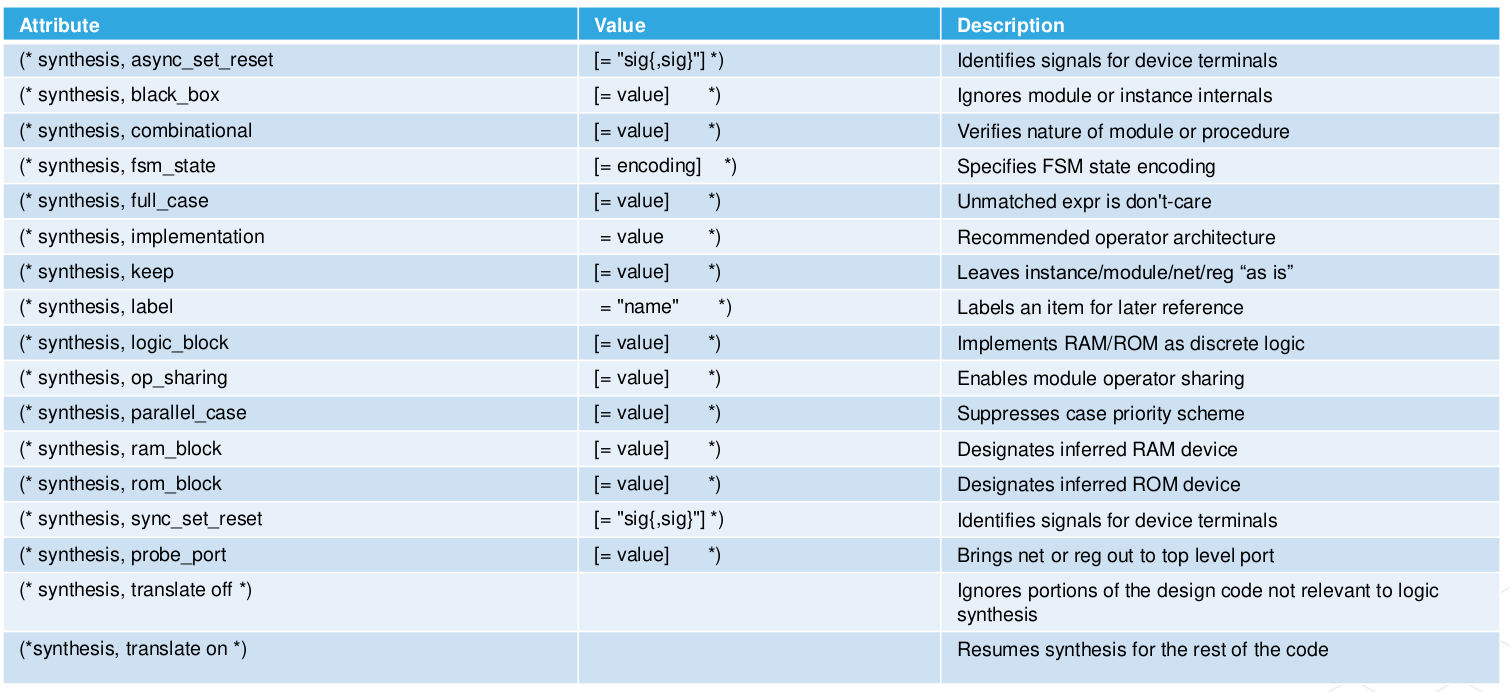
\includegraphics[width=0.95\textwidth]{img/13_reference_attributes.png}
\end{figure}
\end{frame}
\note{
\tiny{

The async\_set\_reset attribute specifies that asynchronous set and reset signals of the module or procedure to which it applies
shall directly connect to the asynchronous set and reset terminals of the library device if the library provides a device with
such terminals. If the attribute specifies signal names, then any other set and reset signals shall not directly connect to
asynchronous set and reset terminals of the device.

The black\_box attribute specifies that synthesis shall ignore the internal contents of the instance or module to which it
applies.

The combinational attribute specifies that synthesis shall report as an error any storage inferred by the module or procedure
to which it applies.

The fsm\_state attribute specifies a state encoding scheme for the register to which it applies.

The full\_case attribute specifies that you don’t care what the outputs are for unspecified case choices.

The implementation attribute recommends an operator architecture.

The keep attribute specifies that synthesis shall preserve an instance, module, net or register “as is”.

The label attribute labels an item for future reference.
The logic\_block attribute supports implementation of a RAM or ROM block in discrete gates.

The op\_sharing attribute can disable operator sharing within a module. Operator sharing may occur anyway without the
attribute. With the attribute enabled, operator sharing may still not occur.
The parallel\_case attribute specifies that synthesis should suppress the normal case statement priority architecture.

The ram\_block attribute supports selection of an inferred RAM device.

The rom\_block attribute supports selection of an inferred ROM device.

The sync\_set\_reset attribute specifies that synchronous set and reset signals of the module or procedure to which it applies
shall directly connect to the synchronous set and reset terminals of the library device if the library provides a device with
such terminals. If the attribute specifies signal names, then any other set and reset signals shall not directly connect to
synchronous set and reset terminals of the device.

The probe\_port attribute causes synthesis to provide a top-level output port connected to the net or
register.

}
}

%%%%%%%%%%%%%%%%%%%%%%%%%%%%%%%%%%%%%%%%%%%%%%%%%%%%%%%%%%%%
\begin{frame}
\frametitle{Reference: Unsupported Verilog Constructs}
\begin{figure}
    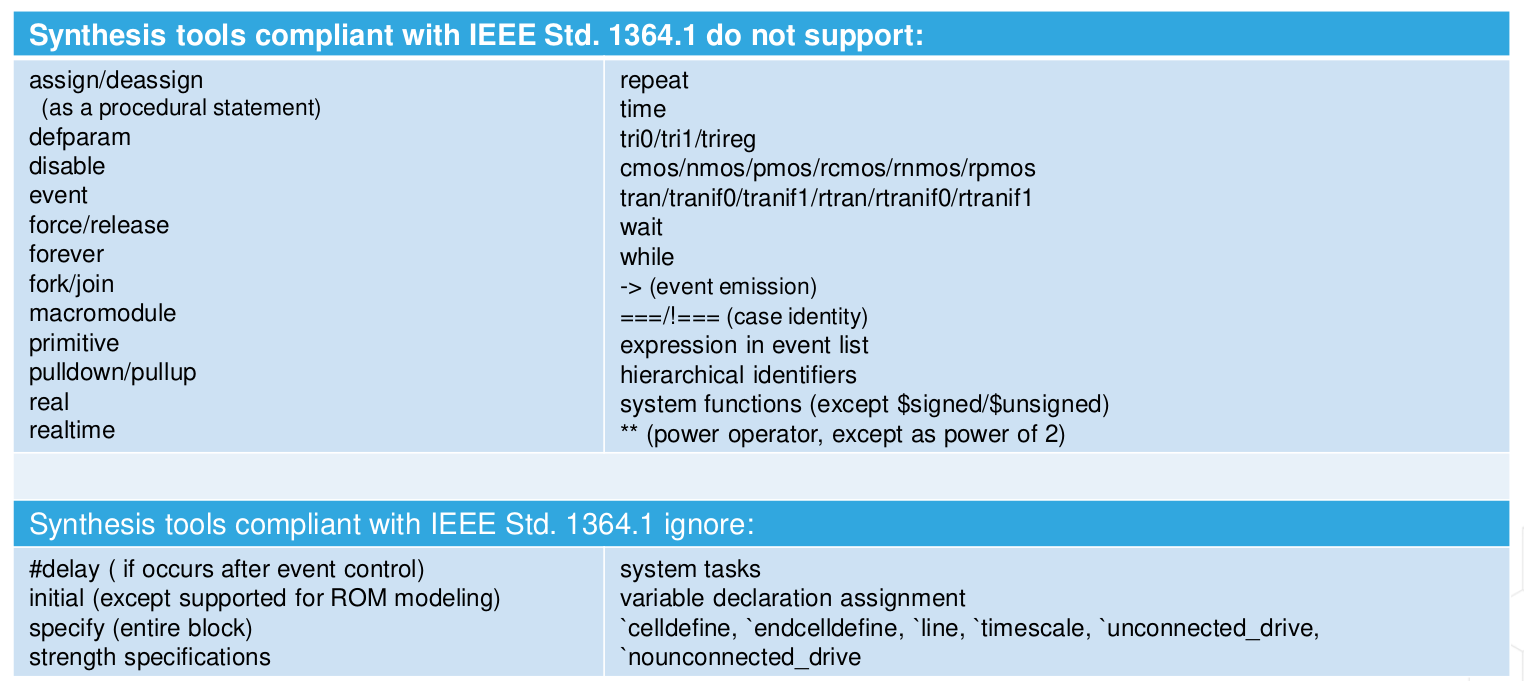
\includegraphics[width=0.95\textwidth]{img/13_unsupported.png}
\end{figure}
\end{frame}
\note{
\scriptsize{
Here for your reference, are constructs that the synthesis tool does not support, and constructs that the synthesis tool ignores.
\newline

Synthesis supports the always keyword only with an immediately following event control (@).

}
}

%%%%%%%%%%%%%%%%%%%%%%%%%%%%%%%%%%%%%%%%%%%%%%%%%%%%%%%%%%%%
\begin{frame}
\frametitle{Module Summary}
\scriptsize{
We should now be able to properly code hardware for logic synthesis.
\newline

This module discussed the following:
\begin{itemize}
\item Modeling combinational logic
\begin{itemize}
	\scriptsize{
	\item In an \textbf{always} block with complete sensitivity list, blocking assignments, and all block outputs assigned each time the
block is executed.
	}
\end{itemize}
\item Modeling sequential logic
\begin{itemize}
	\scriptsize{
	\item In an \textbf{always} block sensitive to edge-qualified events, nonblocking assignments, and set/reset behaviour in early
conditional statement branches.
	}
\end{itemize}
\item Modeling latch logic
\begin{itemize}
	\scriptsize{
	\item By deliberately omitting an output value for some combination of input values.
	}
\end{itemize}
\item Modeling three-state logic
\begin{itemize}
	\scriptsize{
	\item By assigning the high-impedance (Z) state when disabled.
	}
\end{itemize}
\item Using synthesis attributes
\begin{itemize}
	\scriptsize{
	\item E.g., (* synthesis, implementation = "cla" *).
	}
\end{itemize}
\end{itemize}
}
\end{frame}
\note{
\scriptsize{
This module explained how to describe hardware for logic synthesis. It addressed combinational, sequential, latch, and three-state logic. It introduced synthesis attributes that you embed in the source code to influence the synthesis process.

}
}

%%%%%%%%%%%%%%%%%%%%%%%%%%%%%%%%%%%%%%%%%%%%%%%%%%%%%%%%%%%%
\begin{frame}
\frametitle{Module Review}
\scriptsize{
\begin{enumerate}
\item For what conditions does logic synthesis infer a latch in logic you intend to be purely combinational?
\item Explain why a synthesis tool may or may not infer a register for a blocking assignment to a variable.
\item For what Verilog construct does synthesis infer a three-state gate?
\item In what most significant way does synthesis restrict a for loop?
\end{enumerate}
}
\end{frame}
\note{
\scriptsize{
\begin{enumerate}
\item For what conditions does logic synthesis infer a latch in logic you intend to be purely combinational?
\begin{itemize}
	\tiny{
	\item If you fail to specify an output value for at least one combination of input values then logic synthesis will insert a latch.
	}
\end{itemize}
\item Explain why a synthesis tool may or may not infer a register for a blocking assignment to a variable.
\begin{itemize}
	\tiny{
	\item Synthesis infers a register for a blocking assignment to a variable that occurs after the variable is already read in the
execution of a sequential procedure. If the variable is written before it is read then it is only a temporary variable.
	}
\end{itemize}
\item For what Verilog construct does synthesis infer a three-state gate?
\begin{itemize}
	\tiny{
	\item Synthesis infers a three-state gate if you conditionally assign the high-impedance value to a variable.
	}
\end{itemize}
\item In what most significant way does synthesis restrict a for loop?
\begin{itemize}
	\tiny{
	\item You can synthesize a for loop if the number of iterations is a compile-time constant. The synthesis tool unrolls the loop
so needs to know the exact number of iterations.
	}
\end{itemize}
\end{enumerate}

}
}

%%%%%%%%%%%%%%%%%%%%%%%%%%%%%%%%%%%%%%%%%%%%%%%%%%%%%%%%%%%%
\begin{frame}
\frametitle{Module Exercise}
Fix these procedures to make them legal for synthesis:
\begin{figure}
    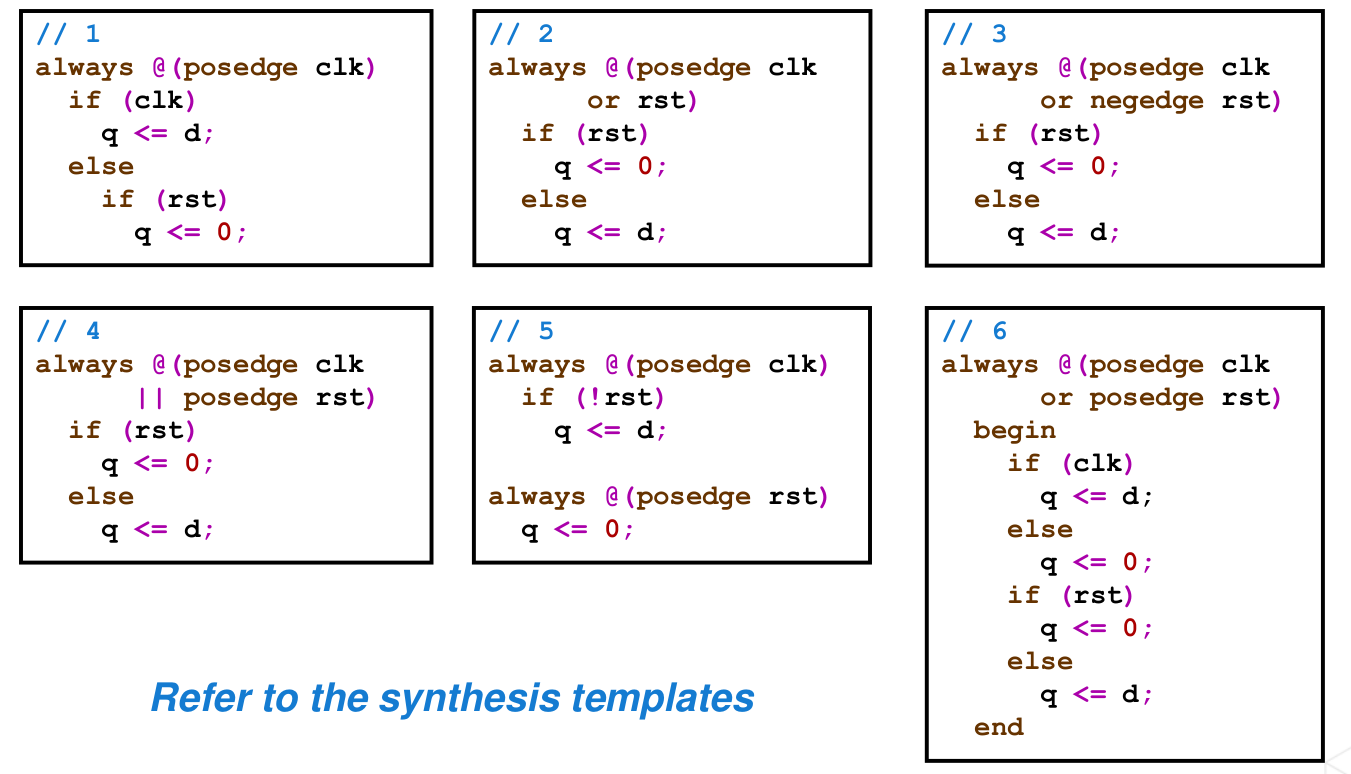
\includegraphics[width=0.95\textwidth]{img/13_ex.png}
\end{figure}
\end{frame}
\note{
\scriptsize{
\begin{figure}
    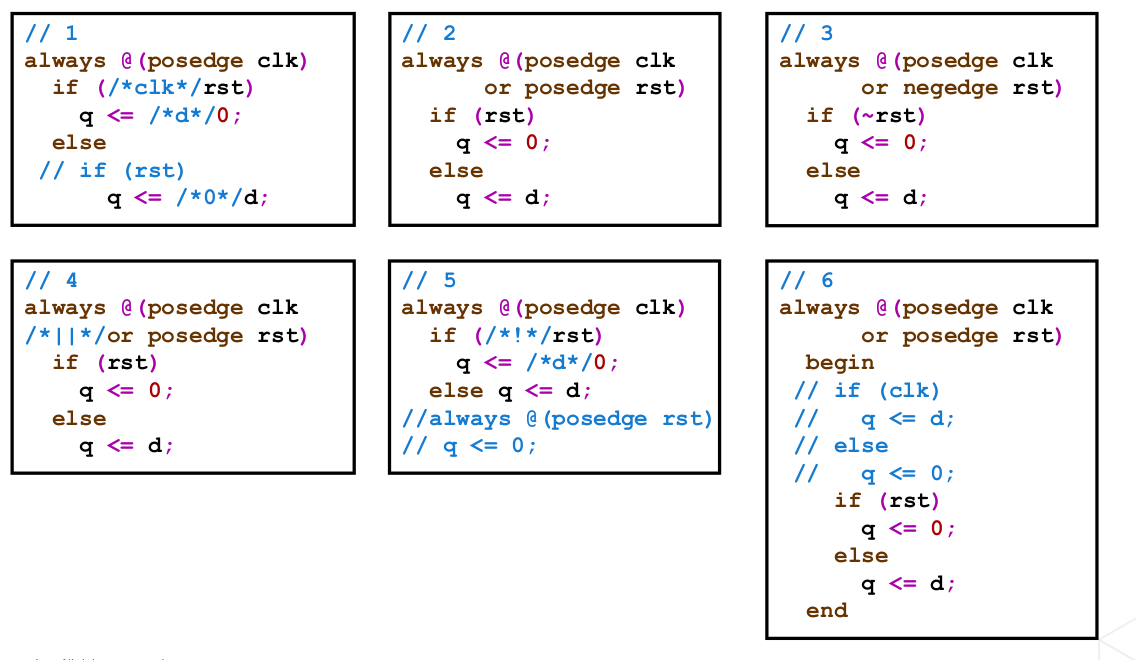
\includegraphics[width=0.95\textwidth]{img/13_ex_sol.png}
\end{figure}

}
}

%%%%%%%%%%%%%%%%%%%%%%%%%%%%%%%%%%%%%%%%%%%%%%%%%%%%%%%%%%%%
\begin{frame}
\frametitle{Lab}
Lab 13-1: Using a Component Library
\begin{itemize}
\item For this Lab, you demonstrate mastery of basic coding styles.
\item And you code and synthesize some representative models.
\end{itemize}
\end{frame}
\note{
\scriptsize{
Your objective for this lab is to describe design behaviour for logic synthesis.
\newline

For this lab, you code and synthesize several simple models and observe the results of different coding
techniques.

}
}



%%%%%%%%%%%%%%%%%%%%%%%%%%%%%%%%%%%%%%%%%%%%%%%%%%%%%%%%%%%%
\begin{frame}
\frametitle{Test You Understanding - 1}
For this piece of your code the synthesis tool infers logic that is:

\ \ always @*
  
\ \ \ \ if(s) y = b;
    
\ \ \ \ else y = a;
\begin{itemize}
\item[$\square$] sequential
\item[$\square$] buffered
\item[$\square$] combinational
\item[$\square$] latched
\item[$\square$] three-state
\end{itemize}
\end{frame}
\note{
\scriptsize{
For this piece of your code the synthesis tool infers logic that is:

\ \ always @*
  
\ \ \ \ if(s) y = b;
    
\ \ \ \ else y = a;
\begin{itemize}
\item[$\square$] sequential
\item[$\square$] buffered
\item[$\boxtimes$] combinational
\item[$\square$] latched
\item[$\square$] three-state
\end{itemize}
}
}

%%%%%%%%%%%%%%%%%%%%%%%%%%%%%%%%%%%%%%%%%%%%%%%%%%%%%%%%%%%%
\begin{frame}
\frametitle{Test You Understanding - 2}
For this piece of your code the synthesis tool infers logic that is:

\ \ always @*
  
\ \ \ \ if(s) y = b;
    
\ \ \ \ else y = 'bz;
\begin{itemize}
\item[$\square$] sequential
\item[$\square$] buffered
\item[$\square$] combinational
\item[$\square$] latched
\item[$\square$] three-state
\end{itemize}
\end{frame}
\note{
\scriptsize{
For this piece of your code the synthesis tool infers logic that is:

\ \ always @*
  
\ \ \ \ if(s) y = b;
    
\ \ \ \ else y = 'bz;
\begin{itemize}
\item[$\square$] sequential
\item[$\square$] buffered
\item[$\square$] combinational
\item[$\square$] latched
\item[$\boxtimes$] three-state
\end{itemize}
}
}


%%%%%%%%%%%%%%%%%%%%%%%%%%%%%%%%%%%%%%%%%%%%%%%%%%%%%%%%%%%%
\begin{frame}
\frametitle{Test You Understanding - 3}

For this piece of your code the synthesis tool infers logic that is:

\ \ always @*
  
\ \ \ \ if(s) y = b;
    
\ \ \ \ else y = 'bx;
\begin{itemize}
\item[$\square$] sequential
\item[$\square$] buffered
\item[$\square$] combinational
\item[$\square$] latched
\end{itemize}
\end{frame}
\note{
\scriptsize{
For this piece of your code the synthesis tool infers logic that is:

\ \ always @*
  
\ \ \ \ if(s) y = b;
    
\ \ \ \ else y = 'bx;
\begin{itemize}
\item[$\square$] sequential
\item[$\boxtimes$] buffered
\item[$\square$] combinational
\item[$\square$] latched
\end{itemize}
}
}

%%%%%%%%%%%%%%%%%%%%%%%%%%%%%%%%%%%%%%%%%%%%%%%%%%%%%%%%%%%%
\begin{frame}
\frametitle{Test You Understanding - 4}
For this piece of your code the synthesis tool infers logic that is:

\ \ always @*
  
\ \ \ \ if(s) y = b;

\begin{itemize}
\item[$\square$] sequential
\item[$\square$] buffered
\item[$\square$] combinational
\item[$\square$] latched
\item[$\square$] three-state
\end{itemize}
\end{frame}
\note{
\scriptsize{
For this piece of your code the synthesis tool infers logic that is:

\ \ always @*
  
\ \ \ \ if(s) y = b;

\begin{itemize}
\item[$\square$] sequential
\item[$\square$] buffered
\item[$\square$] combinational
\item[$\boxtimes$] latched
\item[$\square$] three-state
\end{itemize}
}
}
%%%%%%%%%%%%%%%%%%%%%%%%%%%%%%%%%%%%%%%%%%%%%%%%%%%%%%%%%%%%
\begin{frame}
\frametitle{Test You Understanding - 5}
For this piece of your code the synthesis tool infers logic that is:

\ \ always @(posedge c)
  
\ \ \ \ if(s) y = b;

\begin{itemize}
\item[$\square$] sequential
\item[$\square$] buffered
\item[$\square$] combinational
\item[$\square$] latched
\item[$\square$] three-state
\end{itemize}
\end{frame}
\note{
\scriptsize{
For this piece of your code the synthesis tool infers logic that is:

\ \ always @(posedge c)
  
\ \ \ \ if(s) y = b;

\begin{itemize}
\item[$\boxtimes$] sequential
\item[$\square$] buffered
\item[$\square$] combinational
\item[$\square$] latched
\item[$\square$] three-state
\end{itemize}
}
}



\end{document}
